% !TEX root = ../master-thesis.tex




\begin{figure}
    \centering
    % 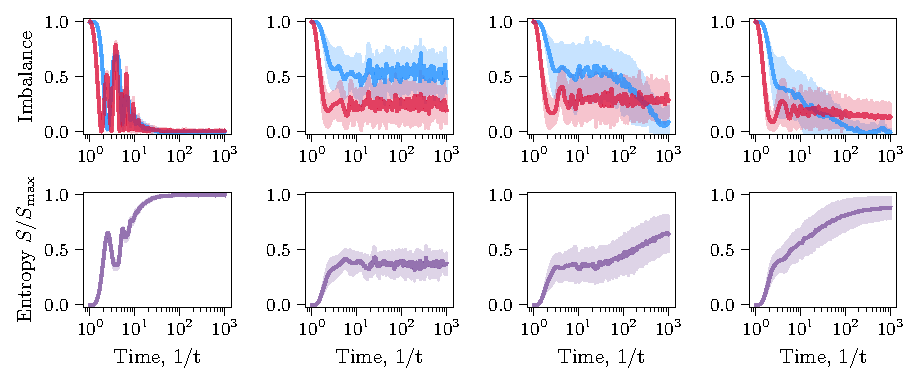
\includegraphics{fig-py/loc-therm.pdf}
    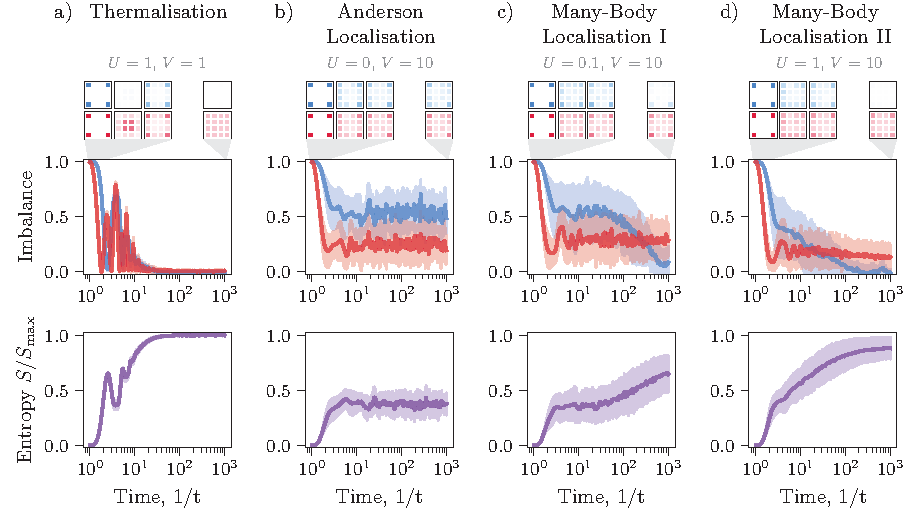
\includegraphics{fig-ai/loc-therm.pdf}
    \caption{
        \textbf{Dynamical phases in a 2D Fermi-Hubbard system.} 
        \textit{Top}: Snapshots of particle density (red) and magnetization magnitude (blue). 
        \textit{Middle}: Time evolution of density imbalance (red) between corners and bulk, and subsystem magnetization (blue). 
        \textit{Bottom}: Normalized entanglement entropy evolution. 
        All results are averaged over 10 noise realizations; shaded areas indicate standard deviation across realizations.
        Data were obtained using ED.
        % Parameters: (a) $U=1, V=1$, (b) $U=0, V=10$, (c) $U=0.1, V=10$, (d) $U=1, V=10$.
        % \\ \textit{Parameters:} (a) $(1,1)$, (b) $(0,10)$, (c) $(0.1,10)$, (d) $(1,10)$ for $(U,V)$.
    }
    \label{fig:loctherm}
\end{figure}

A key application of the numerical simulation toolbox developed in this work is the systematic exploration and clear identification of dynamical phases in interacting fermionic systems, described by the Fermi-Hubbard Hamiltonian. To illustrate this capability, a concrete numerical experiment is considered here, focusing on distinguishing between three distinct dynamical regimes: thermalization governed by Eigenstate Thermalization Hypothesis (ETH), Anderson localization, and many-body localization (MBL). The main motivation for this numerical investigation is to demonstrate explicitly how carefully chosen initial states and targeted observables facilitate clear experimental signatures distinguishing these different phases.

\textbf{Initial state and experimental setup.}
The initial condition selected for this numerical experiment involves a spatially separated arrangement of spin-up and spin-down fermions in a two-dimensional lattice geometry. Specifically, the initial wavefunction is prepared with spin-up fermions localized at two diagonally opposite corners of the lattice, and spin-down fermions positioned at the other two corners. This arrangement generates an initial maximal density imbalance between the corners and the lattice bulk, accompanied by a similarly maximal spin imbalance across the system. This choice of initial condition serves two main purposes. First, it creates a strongly non-equilibrium state that provides clear initial reference points for monitoring relaxation dynamics. Second, it allows separate and simultaneous tracking of particle density and spin distribution, thus providing additional insights into the many-body processes at play.

The Hamiltonian parameters considered in this experiment vary across three physically relevant regimes. In particular, the interaction strength $U$ and disorder strength $V$ are systematically tuned to access the thermalization, Anderson localization, and many-body localization regimes. Simulations are performed using exact diagonalization 
% for moderate system sizes and verified by employing Krylov subspace methods for larger Hilbert-space dimensions. 
For reliable statistics, the results reported in this numerical experiment are averaged over ten independent disorder realizations.

% \begin{figure}
%     \centering
%     % 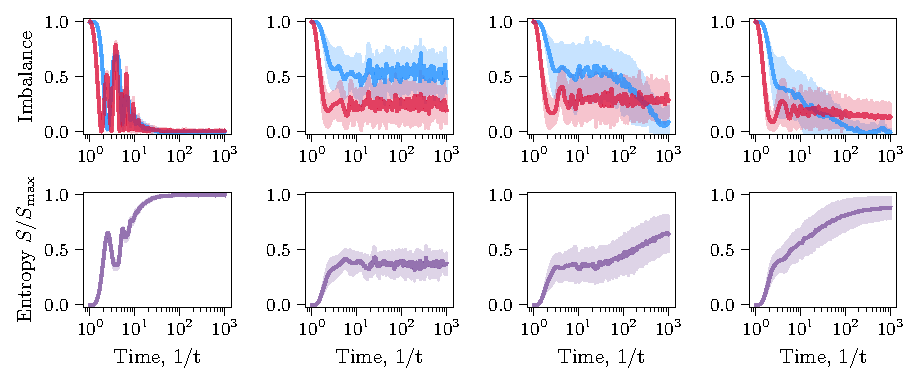
\includegraphics{fig-py/loc-therm.pdf}
%     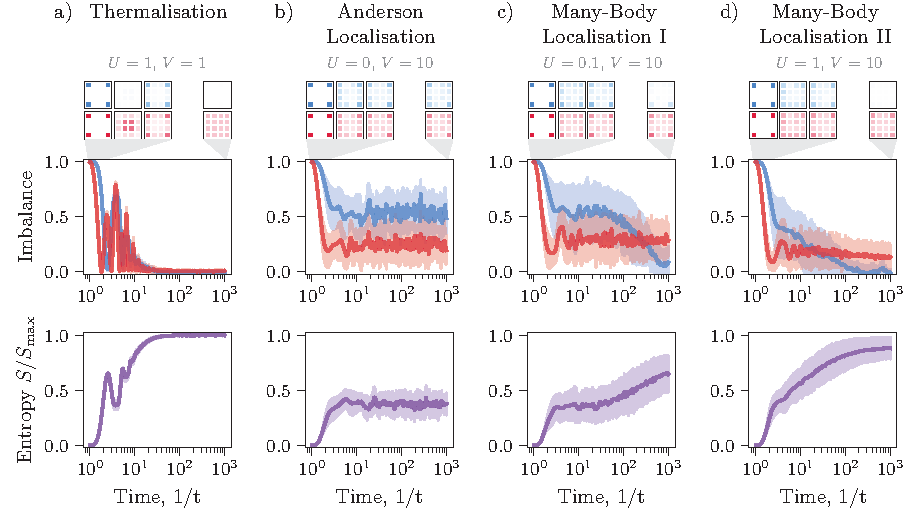
\includegraphics{fig-ai/loc-therm.pdf}
%     \caption{
%         \textbf{Dynamical phases in a 2D Fermi-Hubbard system.} 
%         \textit{Top}: Snapshots of particle density (red) and magnetization magnitude (blue). 
%         \textit{Middle}: Time evolution of density imbalance (red) between corners and bulk, and subsystem magnetization (blue). 
%         \textit{Bottom}: Normalized entanglement entropy evolution. 
%         All results are averaged over 10 noise realizations; shaded areas indicate standard deviation across realizations.
%         Data were obtained using ED.
%         % Parameters: (a) $U=1, V=1$, (b) $U=0, V=10$, (c) $U=0.1, V=10$, (d) $U=1, V=10$.
%         % \\ \textit{Parameters:} (a) $(1,1)$, (b) $(0,10)$, (c) $(0.1,10)$, (d) $(1,10)$ for $(U,V)$.
%     }
%     \label{fig:loctherm}
% \end{figure}


\textbf{Observables and their physical significance.}
Three primary observables are investigated in this numerical experiment to characterize and distinguish among the dynamical phases mentioned above. The first observable is the particle density imbalance, defined as the normalized difference between particle densities at initially occupied corner sites and the bulk sites. Formally, this imbalance can be expressed as
\begin{equation}
\mathcal{I}(t) = \frac{N_\text{corner}(t)-N_\text{bulk}(t)}{N_\text{corner}(t)+N_\text{bulk}(t)},
\end{equation}
where $N_\text{corner}(t)$ and $N_\text{bulk}(t)$ represent particle numbers at corner and bulk sites, respectively, at time $t$. This observable is sensitive to particle redistribution across the lattice, clearly distinguishing thermalization (complete imbalance relaxation), Anderson localization (persistent imbalance), and intermediate behavior in MBL.

The second observable investigated is the subsystem magnetization $\langle \sigma_j^z\rangle$, representing local spin polarization at individual lattice sites. Unlike particle density imbalance alone, magnetization provides further crucial differentiation between Anderson localization, where spin distributions remain essentially static due to absence of interactions, and MBL or thermalization regimes, where spins dynamically rearrange due to interactions.

The third observable employed is the bipartite entanglement entropy, defined by partitioning the lattice system into two equal subsystems. This entropy provides direct insight into the correlation dynamics and quantum information propagation in the system, with characteristic signatures distinctly differentiating ETH, Anderson localization, and MBL phases.

% \textbf{Results and interpretation of numerical simulations.}
The numerical results of this illustrative experiment are summarized in Fig.~\ref{fig:loctherm}. These simulations clearly demonstrate distinct behavior across different regimes, highlighting the utility of the numerical toolbox in characterizing these dynamical phases.


\textbf{Thermalization regime (ETH).}
For parameters corresponding to moderate interaction strength and weak disorder ($U=1$, $V=1$), the numerical results show rapid and complete relaxation of the particle density imbalance to zero, indicating full particle redistribution throughout the lattice. Simultaneously, the subsystem magnetization vanishes on similarly short timescales, clearly reflecting efficient spin mixing driven by interactions. The entanglement entropy exhibits rapid initial growth, quickly reaching saturation at values approaching maximal entropy for the subsystem. These dynamical signatures precisely match theoretical predictions from the ETH framework, wherein local observables lose memory of initial conditions and approach thermodynamic equilibrium at late times \cite{deutsch_quantum_1991,srednicki_chaos_1994}.

\textbf{Anderson localization regime.}
In contrast, the numerical simulations at zero interaction and strong disorder strength ($U=0$, $V=10$) demonstrate distinct dynamical signatures characteristic of Anderson localization. The particle density imbalance remains nearly constant throughout the time evolution, showing negligible redistribution of particles from initial localized positions. Furthermore, subsystem magnetization remains stable, indicating minimal spin rearrangements. Crucially, the entanglement entropy shows almost no growth, stabilizing at values near zero, indicative of the absence of significant entanglement generation. These results clearly align with the theoretical expectation of Anderson localization, where the absence of interactions ensures persistence of initial conditions indefinitely \cite{anderson_absence_1958,abrahams_50_2010}.

\textbf{Many-body localization regime.}
For finite interactions in a strongly disordered environment ($U=0.1$ or $U=1$, with $V=10$), the numerical simulations show the hallmark features of many-body localization. In this regime, the particle imbalance partially relaxes but stabilizes at a finite nonzero value, signifying the suppression but not complete absence of transport. In sharp contrast to Anderson localization, the subsystem magnetization gradually diminishes over time, reflecting slow spin thermalization due to interactions, despite the presence of disorder. Most importantly, the entanglement entropy in this regime exhibits a slow, logarithmic increase without saturating quickly, distinguishing MBL from the other phases clearly. This slow entanglement growth is a distinct theoretical signature of MBL and arises fundamentally from interactions and dephasing processes absent in non-interacting localization scenarios \cite{basko_metalinsulator_2006,nandkishore_many-body_2015}.

% \textbf{Experimental relevance and further perspectives.}
% The presented numerical results clearly illustrate the feasibility of using carefully designed initial states and targeted observables to distinguish experimentally among ETH, Anderson localization, and MBL phases. In particular, the combination of particle density, spin magnetization, and entanglement entropy measurements provides a comprehensive experimental protocol that could be readily implemented in quantum gas microscope experiments or tweezer arrays, such as those considered in the experimental part of this thesis.

% The numerical simulations further guide experimental efforts by predicting observable timescales and characteristic signatures for each phase, thus aiding in the optimal design of measurement protocols. In particular, direct experimental access to local density and spin distributions, combined with recently developed experimental methods for measuring entanglement entropy (e.g., via randomized unitaries), provides a realistic pathway toward direct verification of these theoretical predictions.

% Moreover, the flexibility of the numerical toolbox allows future studies to easily extend these numerical experiments to larger system sizes, different lattice geometries, additional Hamiltonian terms, or modified initial states. Such extensions would significantly enrich the understanding of non-equilibrium quantum dynamics and contribute further to theoretical and experimental explorations of interacting quantum many-body systems.

% In conclusion, this illustrative numerical experiment effectively demonstrates the capability of the developed numerical toolbox to identify and characterize distinct dynamical phases in the Fermi-Hubbard model. Through systematic variation of initial conditions and Hamiltonian parameters, the numerical simulations yield clear and experimentally testable predictions, thus bridging theoretical predictions and experimental realizations in quantum many-body physics.


\textbf{Experimental relevance and further perspectives.}
The presented numerical results illustrate the feasibility of using carefully designed initial states and targeted observables to experimentally distinguish among ETH, Anderson localization, and MBL phases. In particular, simultaneous measurements of particle density, spin magnetization, and entanglement entropy can be directly implemented in experimental setups such as quantum gas microscopes or tweezer arrays, as discussed in previous sections.

Numerical simulations predict characteristic timescales and clear observable signatures for each dynamical phase, providing concrete guidelines for experimental protocols. Furthermore, recently developed experimental methods for measuring entanglement entropy, such as randomized unitaries, offer realistic pathways for direct verification of theoretical predictions.







